% =====================================================================
%  Capítulo 8. Modelos ARCH y GARCH
% =====================================================================
\part{Volatilidad}
\chapter[Modelos ARCH y GARCH]{Volatilidad condicional: modelos ARCH y GARCH}\label{cap:garch}

\section*{Objetivos de aprendizaje}
Al terminar este capítulo, el lector podrá:
\begin{enumerate}[label=\arabic*.,leftmargin=*]
  \item Derivar los momentos de los procesos ARCH(1) y GARCH(1,1), en particular su varianza incondicional y
        su curtosis, y explicar por qué generan colas gruesas y agrupamiento de volatilidad.
  \item Detectar efectos ARCH con la prueba de Ljung-Box sobre los cuadrados y la prueba LM de Engle.
  \item Programar y maximizar la verosimilitud de un GARCH(1,1) con innovaciones normales y $t$ de Student, y
        calcular errores estándar robustos de cuasi máxima verosimilitud.
  \item Pronosticar la varianza a varios horizontes, calcular la vida media de los choques y evaluar los
        pronósticos fuera de muestra con funciones de pérdida apropiadas.
\end{enumerate}

\section*{Motivación}
El Capítulo~\ref{cap:hechos} mostró que los rendimientos casi no están autocorrelacionados, pero sus cuadrados
sí: los días agitados vienen juntos y los tranquilos también. El Capítulo~\ref{cap:robustos} trató esa
heterocedasticidad como un estorbo para la inferencia; el Capítulo~\ref{cap:eficiencia}, como una razón para
usar pruebas robustas. Este capítulo la convierte en el objeto de estudio. La volatilidad no se observa, pero
es predecible, y su pronóstico es la materia prima de la gestión de riesgos (valor en riesgo, Capítulo~13), de
la valoración de opciones y de la asignación de carteras. Engle (1982) propuso el modelo ARCH para la inflación
británica; Bollerslev (1986) lo generalizó al GARCH, que sigue siendo el modelo de referencia.

\paragraph{Datos del capítulo.} Rendimientos logarítmicos diarios del Brent en porcentaje (mayo de 1987 a
noviembre de 2026, $T=9\,121$) y rendimientos mensuales del S\&P 500 (base de Shiller, 1871--2026). Expresar
los rendimientos en porcentaje (multiplicar por 100) no cambia nada sustantivo, pero evita que $\omega$ sea un
número del orden de $10^{-6}$, lo que dificulta la optimización numérica.

% ---------------------------------------------------------------------
\section{El modelo ARCH}
% ---------------------------------------------------------------------

Escribimos el rendimiento como su media condicional más una innovación,
\[
  r_t=\mu+\varepsilon_t,\qquad \varepsilon_t=\sigma_t z_t,\qquad z_t\sim\text{i.i.d.}(0,1),
\]
donde $\sigma_t$ depende solo de la información hasta $t-1$. Entonces
$\E[\varepsilon_t\mid\mathcal F_{t-1}]=\sigma_t\E[z_t]=0$ y
$\Var(\varepsilon_t\mid\mathcal F_{t-1})=\sigma_t^2\E[z_t^2]=\sigma_t^2$: $\sigma_t^2$ es la \emph{varianza
condicional}.

\begin{definicion}[ARCH($q$); Engle, 1982]
La innovación sigue un proceso autorregresivo condicionalmente heterocedástico de orden $q$ si
\[
  \sigma_t^2=\omega+\alpha_1\varepsilon_{t-1}^2+\dots+\alpha_q\varepsilon_{t-q}^2,
  \qquad \omega>0,\ \alpha_i\ge0 .
\]
\end{definicion}

Un rendimiento grande hoy, de cualquier signo, eleva la varianza de mañana; eso produce agrupamiento de
volatilidad. Las restricciones de signo garantizan que $\sigma_t^2>0$.

\begin{proposicion}[Propiedades del ARCH(1)]\label{prop:arch1}
Sea $\sigma_t^2=\omega+\alpha\varepsilon_{t-1}^2$ con $z_t\sim N(0,1)$ y $0\le\alpha<1$. Entonces:
\begin{enumerate}[label=(\roman*)]
  \item $\varepsilon_t$ no está autocorrelacionado;
  \item su varianza incondicional es $\sigma^2=\omega/(1-\alpha)$;
  \item $\varepsilon_t^2$ sigue un AR(1): $\varepsilon_t^2=\omega+\alpha\varepsilon_{t-1}^2+v_t$, con
        $\E[v_t\mid\mathcal F_{t-1}]=0$;
  \item si $3\alpha^2<1$, la curtosis es $\kappa=3(1-\alpha^2)/(1-3\alpha^2)>3$.
\end{enumerate}
\end{proposicion}

\begin{proof}
(i) Como $\E[\varepsilon_t\mid\mathcal F_{t-1}]=0$, la Proposición~\ref{prop:martingala} con $g=\varepsilon_{t-j}$
da $\Cov(\varepsilon_t,\varepsilon_{t-j})=0$ para $j\ge1$.

(ii) Por la ley de esperanzas iteradas, y usando la estacionariedad ($\E[\varepsilon_t^2]=\E[\varepsilon_{t-1}^2]=\sigma^2$):
\begin{align*}
  \E[\varepsilon_t^2] &= \E\bigl[\E[\sigma_t^2z_t^2\mid\mathcal F_{t-1}]\bigr]\\
                      &= \E[\sigma_t^2]\\
                      &= \omega+\alpha\,\E[\varepsilon_{t-1}^2],\\[4pt]
  \sigma^2            &= \omega+\alpha\,\sigma^2,\\
  \sigma^2(1-\alpha)  &= \omega,\\
  \sigma^2            &= \frac{\omega}{1-\alpha}.
\end{align*}

(iii) Definimos $v_t=\varepsilon_t^2-\sigma_t^2$. Entonces
\begin{align*}
  \varepsilon_t^2 &= \sigma_t^2+v_t\\
                  &= \omega+\alpha\varepsilon_{t-1}^2+v_t,\\[4pt]
  \E[v_t\mid\mathcal F_{t-1}] &= \E[\varepsilon_t^2\mid\mathcal F_{t-1}]-\sigma_t^2\\
                              &= \sigma_t^2-\sigma_t^2\\
                              &= 0 .
\end{align*}

(iv) Con $z_t$ normal, $\E[z_t^4]=3$. Sea $m_4=\E[\varepsilon_t^4]$, igual para todo $t$ por estacionariedad:
\begin{align*}
  m_4 &= \E[\sigma_t^4z_t^4]\\
      &= 3\,\E[\sigma_t^4]\\
      &= 3\,\E\bigl[(\omega+\alpha\varepsilon_{t-1}^2)^2\bigr]\\
      &= 3\bigl(\omega^2+2\omega\alpha\,\E[\varepsilon_{t-1}^2]+\alpha^2\E[\varepsilon_{t-1}^4]\bigr)\\
      &= 3\omega^2+6\omega\alpha\sigma^2+3\alpha^2m_4 .
\end{align*}
Despejamos $m_4$ y usamos $\omega=\sigma^2(1-\alpha)$:
\begin{align*}
  m_4(1-3\alpha^2) &= 3\omega^2+6\omega\alpha\sigma^2\\
                   &= 3\omega(\omega+2\alpha\sigma^2)\\
                   &= 3\sigma^2(1-\alpha)\bigl[\sigma^2(1-\alpha)+2\alpha\sigma^2\bigr]\\
                   &= 3\sigma^4(1-\alpha)(1+\alpha)\\
                   &= 3\sigma^4(1-\alpha^2).
\end{align*}
Dividiendo entre $\sigma^4(1-3\alpha^2)$, que es positivo si $3\alpha^2<1$:
\begin{align*}
  \kappa &= \frac{m_4}{\sigma^4}\\
         &= \frac{3(1-\alpha^2)}{1-3\alpha^2}.
\end{align*}
Como $1-\alpha^2>1-3\alpha^2$ cuando $\alpha>0$, el cociente es mayor que uno y $\kappa>3$.
\end{proof}

La parte (iv) es notable: aunque cada $z_t$ es normal, la distribución \emph{incondicional} de $\varepsilon_t$
tiene colas más gruesas que la normal, porque es una mezcla de normales con varianzas distintas. Con
$\omega=0{,}5$ y $\alpha=0{,}5$ la varianza incondicional es $0{,}5/0{,}5=1$ y
\begin{align*}
  \kappa &= \frac{3(1-0{,}25)}{1-0{,}75}\\
         &= \frac{2{,}25}{0{,}25}\\
         &= 9 .
\end{align*}
La Figura~\ref{fig:archsim} compara una trayectoria de ese proceso con ruido normal de la misma varianza: el
ARCH alterna tramos tranquilos y ráfagas de valores extremos, y su densidad (estimada con 400\,000
simulaciones, cuya curtosis muestral es $9{,}67$) tiene más pico y colas mucho más altas que la normal.

\begin{figure}[ht]
\centering
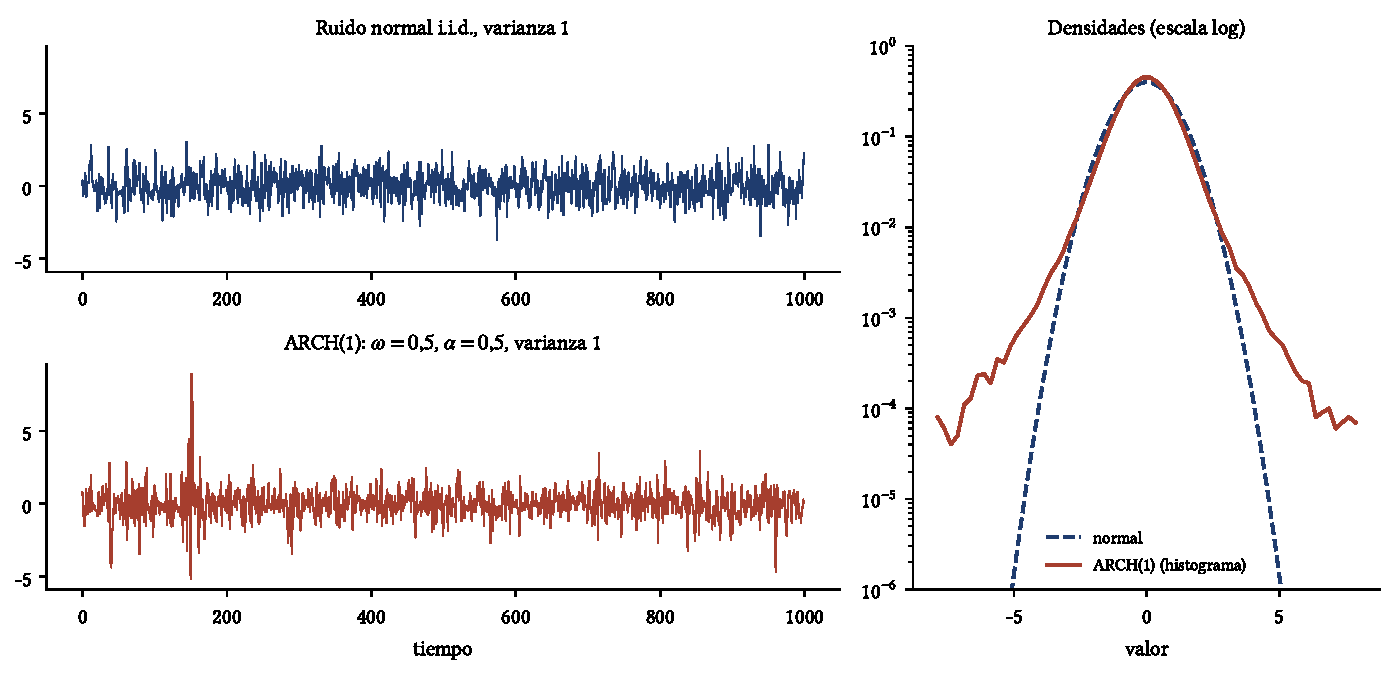
\includegraphics[width=\linewidth]{graficos/cap08_fig_arch_sim.pdf}
\caption{Izquierda: ruido normal i.i.d.\ y un ARCH(1) con $\omega=\alpha=0{,}5$, ambos con varianza
incondicional 1. Derecha: densidad del ARCH(1) frente a la normal en escala logarítmica; las colas del ARCH
caen mucho más despacio.}
\label{fig:archsim}
\end{figure}

% ---------------------------------------------------------------------
\section{El modelo GARCH}
% ---------------------------------------------------------------------

En la práctica, un ARCH necesita muchos rezagos para reproducir la persistencia de la volatilidad. Bollerslev
(1986) agregó la varianza rezagada a la ecuación.

\begin{definicion}[GARCH(1,1)]
\[
  \sigma_t^2=\omega+\alpha\,\varepsilon_{t-1}^2+\beta\,\sigma_{t-1}^2,\qquad
  \omega>0,\ \alpha\ge0,\ \beta\ge0 .
\]
\end{definicion}

La varianza de mañana es un promedio ponderado de un nivel de largo plazo, la ``noticia'' de hoy
($\varepsilon_{t-1}^2$) y la varianza de hoy. El coeficiente $\alpha$ mide la reacción a las noticias y
$\beta$ la inercia.

\begin{proposicion}[Representación ARCH($\infty$)]\label{prop:archinf}
Si $0\le\beta<1$,
\[
  \sigma_t^2=\frac{\omega}{1-\beta}+\alpha\sum_{j=1}^{\infty}\beta^{\,j-1}\varepsilon_{t-j}^2 .
\]
\end{proposicion}

\begin{proof}
Sustituimos la ecuación del GARCH en sí misma para $\sigma_{t-1}^2$, luego para $\sigma_{t-2}^2$, y así
sucesivamente:
\begin{align*}
  \sigma_t^2 &= \omega+\alpha\varepsilon_{t-1}^2+\beta\sigma_{t-1}^2\\
             &= \omega+\alpha\varepsilon_{t-1}^2+\beta\bigl(\omega+\alpha\varepsilon_{t-2}^2+\beta\sigma_{t-2}^2\bigr)\\
             &= \omega(1+\beta)+\alpha\bigl(\varepsilon_{t-1}^2+\beta\varepsilon_{t-2}^2\bigr)+\beta^2\sigma_{t-2}^2\\
             &\;\;\vdots\\
             &= \omega\sum_{j=0}^{k-1}\beta^j+\alpha\sum_{j=1}^{k}\beta^{\,j-1}\varepsilon_{t-j}^2+\beta^k\sigma_{t-k}^2 .
\end{align*}
Cuando $k\to\infty$, $\beta^k\sigma_{t-k}^2\to0$ y la serie geométrica converge:
\begin{align*}
  \omega\sum_{j=0}^{\infty}\beta^j &= \frac{\omega}{1-\beta}. && \qedhere
\end{align*}
\end{proof}

El GARCH(1,1) es entonces un ARCH de orden infinito con pesos que decrecen geométricamente: con solo tres
parámetros recuerda todo el pasado.

\begin{proposicion}[Momentos del GARCH(1,1)]\label{prop:garchmom}
Si $\alpha+\beta<1$:
\begin{enumerate}[label=(\roman*)]
  \item la varianza incondicional es $\bar\sigma^2=\omega/(1-\alpha-\beta)$;
  \item $\varepsilon_t^2$ sigue un ARMA(1,1):
        $\varepsilon_t^2=\omega+(\alpha+\beta)\varepsilon_{t-1}^2+v_t-\beta v_{t-1}$, con
        $v_t=\varepsilon_t^2-\sigma_t^2$;
  \item con $z_t$ normal y $(\alpha+\beta)^2+2\alpha^2<1$, la curtosis es
        \[
          \kappa=\frac{3\bigl[1-(\alpha+\beta)^2\bigr]}{1-(\alpha+\beta)^2-2\alpha^2}>3 .
        \]
\end{enumerate}
\end{proposicion}

\begin{proof}
(i) Tomamos esperanzas en la ecuación del GARCH, con $\E[\varepsilon_{t-1}^2]=\E[\sigma_{t-1}^2]=\bar\sigma^2$:
\begin{align*}
  \bar\sigma^2 &= \omega+\alpha\bar\sigma^2+\beta\bar\sigma^2,\\
  \bar\sigma^2(1-\alpha-\beta) &= \omega,\\
  \bar\sigma^2 &= \frac{\omega}{1-\alpha-\beta}.
\end{align*}

(ii) Sustituimos $\sigma_t^2=\varepsilon_t^2-v_t$ y $\sigma_{t-1}^2=\varepsilon_{t-1}^2-v_{t-1}$:
\begin{align*}
  \varepsilon_t^2-v_t &= \omega+\alpha\varepsilon_{t-1}^2+\beta\bigl(\varepsilon_{t-1}^2-v_{t-1}\bigr),\\
  \varepsilon_t^2     &= \omega+(\alpha+\beta)\varepsilon_{t-1}^2+v_t-\beta v_{t-1}.
\end{align*}

(iii) Escribimos la recursión en función de $z_{t-1}$, usando $\varepsilon_{t-1}^2=\sigma_{t-1}^2z_{t-1}^2$:
\begin{align*}
  \sigma_t^2 &= \omega+\sigma_{t-1}^2\bigl(\alpha z_{t-1}^2+\beta\bigr).
\end{align*}
Como $z_{t-1}$ es independiente de $\sigma_{t-1}^2$, con $\E[z^2]=1$ y $\E[z^4]=3$:
\begin{align*}
  \E\bigl[(\alpha z^2+\beta)^2\bigr] &= \alpha^2\E[z^4]+2\alpha\beta\E[z^2]+\beta^2\\
                                     &= 3\alpha^2+2\alpha\beta+\beta^2\\
                                     &= (\alpha+\beta)^2+2\alpha^2 .
\end{align*}
Llamamos $c=(\alpha+\beta)^2+2\alpha^2$ y $m=\E[\sigma_t^4]$. Elevamos al cuadrado y tomamos esperanzas:
\begin{align*}
  m &= \omega^2+2\omega\,\E[\sigma_{t-1}^2]\,\E[\alpha z^2+\beta]+\E[\sigma_{t-1}^4]\,\E\bigl[(\alpha z^2+\beta)^2\bigr]\\
    &= \omega^2+2\omega\bar\sigma^2(\alpha+\beta)+c\,m,\\[4pt]
  m(1-c) &= \omega^2+2\omega\bar\sigma^2(\alpha+\beta).
\end{align*}
Con $\omega=\bar\sigma^2(1-\alpha-\beta)$, el lado derecho es
\begin{align*}
  \omega\bigl[\omega+2\bar\sigma^2(\alpha+\beta)\bigr]
    &= \bar\sigma^2(1-\alpha-\beta)\,\bar\sigma^2\bigl[(1-\alpha-\beta)+2(\alpha+\beta)\bigr]\\
    &= \bar\sigma^4(1-\alpha-\beta)(1+\alpha+\beta)\\
    &= \bar\sigma^4\bigl[1-(\alpha+\beta)^2\bigr].
\end{align*}
Finalmente, $\E[\varepsilon_t^4]=\E[\sigma_t^4]\E[z_t^4]=3m$, y si $c<1$:
\begin{align*}
  \kappa &= \frac{3m}{\bar\sigma^4}\\
         &= \frac{3\bigl[1-(\alpha+\beta)^2\bigr]}{1-c}\\
         &= \frac{3\bigl[1-(\alpha+\beta)^2\bigr]}{1-(\alpha+\beta)^2-2\alpha^2}.
\end{align*}
El denominador es menor que el término entre corchetes cuando $\alpha>0$, así que $\kappa>3$.
\end{proof}

La parte (ii) explica la forma de la ACF de los cuadrados: decae geométricamente a la tasa $\alpha+\beta$, que
se llama \emph{persistencia}. La parte (iii) impone una condición más exigente que la estacionariedad. La
Figura~\ref{fig:region} dibuja las dos regiones en el plano $(\alpha,\beta)$: debajo de la recta
$\alpha+\beta=1$ el proceso es estacionario, pero solo debajo de la curva $(\alpha+\beta)^2+2\alpha^2=1$ tiene
cuarto momento finito. Las estimaciones típicas con datos diarios (una $\alpha$ pequeña y una $\beta$ cercana a
uno) caen en la franja intermedia, muy cerca de la recta: varianza finita, pero curtosis infinita.

\begin{figure}[ht]
\centering
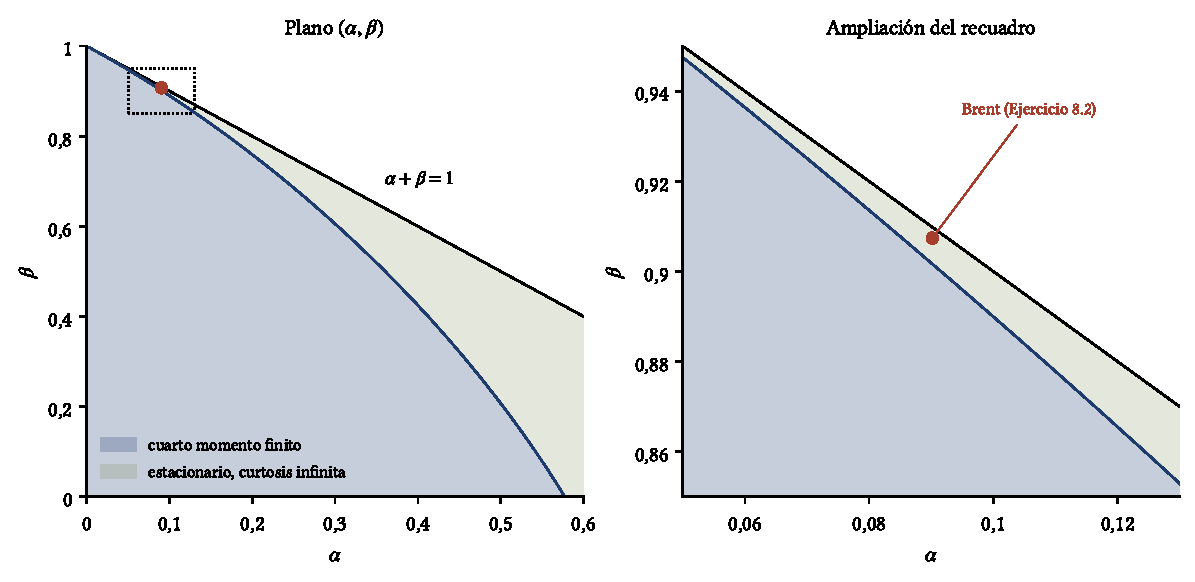
\includegraphics[width=\linewidth]{graficos/cap08_fig_region.pdf}
\caption{Regiones del GARCH(1,1) con innovaciones normales. Azul: estacionario con cuarto momento finito.
Verde claro: estacionario con curtosis infinita. El punto rojo es la estimación del Ejercicio~\ref{ej:garchn}
para el Brent, que cae en la franja de curtosis infinita.}
\label{fig:region}
\end{figure}

\paragraph{IGARCH y EWMA.} Si $\alpha+\beta=1$, el modelo es un GARCH \emph{integrado} (IGARCH): los choques
a la varianza no se disipan y la varianza incondicional no existe. El caso particular con $\omega=0$,
$\alpha=1-\lambda$ y $\beta=\lambda$,
\[
  \sigma_t^2=\lambda\,\sigma_{t-1}^2+(1-\lambda)\,\varepsilon_{t-1}^2,
\]
es la \emph{media móvil ponderada exponencialmente} (EWMA) que popularizó RiskMetrics (J.\,P.~Morgan, 1996)
con $\lambda=0{,}94$ para datos diarios. No se estima: se fija $\lambda$.

% ---------------------------------------------------------------------
\section{Pronóstico de la varianza}
% ---------------------------------------------------------------------

\begin{proposicion}[Pronóstico del GARCH(1,1)]\label{prop:garchpron}
Sea $\phi=\alpha+\beta<1$ y $\E_T[\cdot]=\E[\cdot\mid\mathcal F_T]$. La varianza de $T+1$ se conoce en $T$, y
para $h\ge1$
\[
  \E_T\bigl[\sigma_{T+h}^2\bigr]=\bar\sigma^2+\phi^{\,h-1}\bigl(\sigma_{T+1}^2-\bar\sigma^2\bigr).
\]
\end{proposicion}

\begin{proof}
Para $h=1$ la fórmula da $\sigma_{T+1}^2$, que es conocida en $T$. Supongamos que vale para $h-1\ge1$. Como
$\E_T[\varepsilon_{T+h-1}^2]=\E_T\bigl[\E_{T+h-2}[\sigma_{T+h-1}^2z_{T+h-1}^2]\bigr]=\E_T[\sigma_{T+h-1}^2]$,
\begin{align*}
  \E_T\bigl[\sigma_{T+h}^2\bigr]
    &= \omega+\alpha\,\E_T[\varepsilon_{T+h-1}^2]+\beta\,\E_T[\sigma_{T+h-1}^2]\\
    &= \omega+(\alpha+\beta)\,\E_T[\sigma_{T+h-1}^2]\\
    &= \omega+\phi\bigl[\bar\sigma^2+\phi^{\,h-2}(\sigma_{T+1}^2-\bar\sigma^2)\bigr]\\
    &= \omega+\phi\bar\sigma^2+\phi^{\,h-1}(\sigma_{T+1}^2-\bar\sigma^2).
\end{align*}
Por la Proposición~\ref{prop:garchmom}, $\omega=\bar\sigma^2(1-\phi)$, así que
\begin{align*}
  \omega+\phi\bar\sigma^2 &= \bar\sigma^2-\phi\bar\sigma^2+\phi\bar\sigma^2\\
                          &= \bar\sigma^2,
\end{align*}
y la fórmula vale para $h$. Por inducción, vale para todo $h\ge1$.
\end{proof}

El pronóstico converge geométricamente a $\bar\sigma^2$, desde arriba si hoy la volatilidad está alta y desde
abajo si está baja (Figura~\ref{fig:pronteo}). La rapidez depende solo de la persistencia. La \emph{vida media}
de un choque, el horizonte en que la mitad de la desviación respecto de $\bar\sigma^2$ ha desaparecido, resulta
de
\begin{align*}
  \phi^{\,h} &= \tfrac12,\\
  h\ln\phi   &= \ln\tfrac12,\\
  h          &= \frac{\ln 0{,}5}{\ln\phi}.
\end{align*}
Con $\phi=0{,}97$ la vida media es de 22,8 días; con $\phi=0{,}995$, de 138,3 días.

\begin{figure}[ht]
\centering
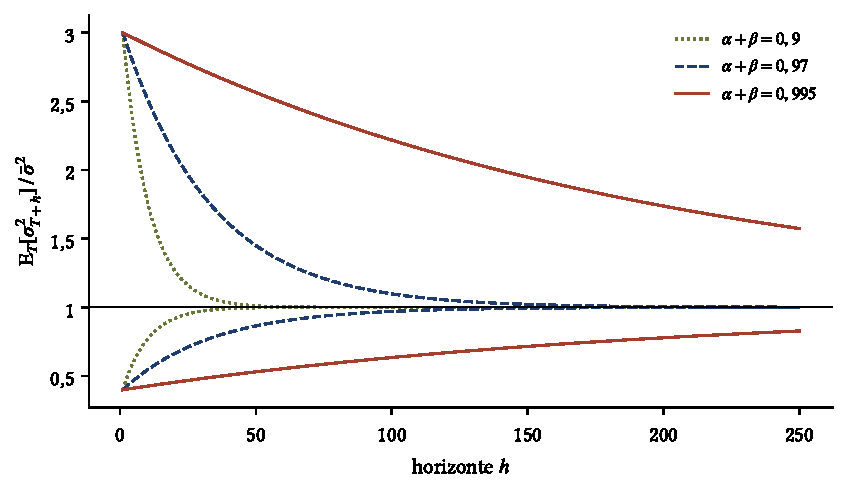
\includegraphics[width=0.74\linewidth]{graficos/cap08_fig_pronostico_teo.pdf}
\caption{Pronóstico de la varianza relativo a su nivel incondicional, partiendo de una varianza tres veces
mayor (curvas superiores) o un 60\,\% menor (inferiores). Cuanto mayor la persistencia $\alpha+\beta$, más lenta
la convergencia.}
\label{fig:pronteo}
\end{figure}

\begin{corolario}[Varianza de un rendimiento de $H$ períodos]\label{cor:varH}
Como los rendimientos no están correlacionados, la varianza condicional del rendimiento acumulado de $T+1$ a
$T+H$ es la suma de las varianzas pronosticadas:
\[
  \sum_{h=1}^{H}\E_T\bigl[\sigma_{T+h}^2\bigr]=H\bar\sigma^2+\bigl(\sigma_{T+1}^2-\bar\sigma^2\bigr)\frac{1-\phi^H}{1-\phi}.
\]
\end{corolario}

\begin{proof}
Sumamos la fórmula de la Proposición~\ref{prop:garchpron}:
\begin{align*}
  \sum_{h=1}^{H}\E_T\bigl[\sigma_{T+h}^2\bigr]
     &= \sum_{h=1}^{H}\bar\sigma^2+\bigl(\sigma_{T+1}^2-\bar\sigma^2\bigr)\sum_{h=1}^{H}\phi^{\,h-1}\\
     &= H\bar\sigma^2+\bigl(\sigma_{T+1}^2-\bar\sigma^2\bigr)\bigl(1+\phi+\dots+\phi^{H-1}\bigr)\\
     &= H\bar\sigma^2+\bigl(\sigma_{T+1}^2-\bar\sigma^2\bigr)\frac{1-\phi^H}{1-\phi}. && \qedhere
\end{align*}
\end{proof}

La regla de la raíz del tiempo del Capítulo~\ref{cap:rendimientos}, $\sqrt{H}\,\sigma_{T+1}$, supone que la
varianza de hoy se mantiene. Si la volatilidad está alta, la regla sobreestima el riesgo de horizonte largo;
si está baja, lo subestima.

% ---------------------------------------------------------------------
\section{Estimación por máxima verosimilitud}
% ---------------------------------------------------------------------

\subsection{La verosimilitud}
La densidad conjunta de la muestra se factoriza en densidades condicionales sucesivas:
\begin{align*}
  f(r_1,\dots,r_T) &= f(r_1)\,f(r_2\mid r_1)\cdots f(r_T\mid r_1,\dots,r_{T-1})\\
                   &= \prod_{t=1}^{T}f(r_t\mid\mathcal F_{t-1}).
\end{align*}
Con $z_t$ normal, $r_t\mid\mathcal F_{t-1}\sim N(\mu,\sigma_t^2)$, y el logaritmo de la verosimilitud es
\begin{align*}
  \ell(\theta) &= \sum_{t=1}^{T}\ell_t(\theta),\\
  \ell_t(\theta) &= -\frac12\Bigl[\ln(2\pi)+\ln\sigma_t^2+\frac{(r_t-\mu)^2}{\sigma_t^2}\Bigr],
\end{align*}
con $\theta=(\mu,\omega,\alpha,\beta)$ y $\sigma_t^2$ calculada con la recursión del GARCH. La recursión
necesita un valor inicial; usamos el de la biblioteca \texttt{arch}, un promedio con pesos $0{,}94^{\,j}$ de los
primeros 75 cuadrados de los residuos (\emph{backcast}). No hay fórmula cerrada para el máximo: se maximiza
numéricamente con las restricciones $\omega>0$, $\alpha,\beta\ge0$.

\subsection{Innovaciones $t$ de Student}
Aun después de dividir entre $\sigma_t$, los residuos de los rendimientos financieros suelen tener colas más
gruesas que la normal. Una alternativa es suponer que $z_t$ sigue una $t$ de Student con $\nu>2$ grados de
libertad, reescalada para que su varianza sea 1.

\begin{proposicion}[$t$ de Student estandarizada]\label{prop:tstd}
Si $X\sim t_\nu$ con $\nu>2$, $\Var(X)=\nu/(\nu-2)$. Por tanto $z=X\sqrt{(\nu-2)/\nu}$ tiene varianza 1 y
densidad
\[
  f(z)=\frac{\Gamma\bigl(\frac{\nu+1}2\bigr)}{\Gamma\bigl(\frac\nu2\bigr)\sqrt{\pi(\nu-2)}}
       \Bigl(1+\frac{z^2}{\nu-2}\Bigr)^{-\frac{\nu+1}2}.
\]
Si $\nu>4$, su curtosis es $3+6/(\nu-4)$.
\end{proposicion}

\begin{proof}
La varianza de la $t_\nu$ y su curtosis $3+6/(\nu-4)$ son resultados estándar. Para el reescalamiento,
\begin{align*}
  \Var(z) &= \frac{\nu-2}{\nu}\,\Var(X)\\
          &= \frac{\nu-2}{\nu}\cdot\frac{\nu}{\nu-2}\\
          &= 1 .
\end{align*}
La curtosis no cambia al multiplicar por una constante. Para la densidad, con $c=\sqrt{(\nu-2)/\nu}$ y $x=z/c$,
el cambio de variable da $f_z(z)=f_X(z/c)/c$. Como
\begin{align*}
  \frac{x^2}{\nu} &= \frac{z^2}{c^2\nu}\\
                  &= \frac{z^2}{\nu-2},\\[4pt]
  c\sqrt{\nu\pi}  &= \sqrt{\frac{\nu-2}{\nu}}\sqrt{\nu\pi}\\
                  &= \sqrt{\pi(\nu-2)},
\end{align*}
al sustituir en la densidad de la $t_\nu$ se obtiene la fórmula del enunciado.
\end{proof}

La contribución de cada observación a la log-verosimilitud, con $z_t=(r_t-\mu)/\sigma_t$, es
\begin{align*}
  \ell_t &= \ln\Gamma\Bigl(\frac{\nu+1}{2}\Bigr)-\ln\Gamma\Bigl(\frac\nu2\Bigr)-\frac12\ln\bigl[\pi(\nu-2)\bigr]
            -\frac12\ln\sigma_t^2-\frac{\nu+1}{2}\ln\Bigl(1+\frac{z_t^2}{\nu-2}\Bigr),
\end{align*}
donde el término $-\frac12\ln\sigma_t^2$ es el jacobiano de pasar de $z_t$ a $r_t$. La
Figura~\ref{fig:tstudentstd} compara la $t$ estandarizada con la normal: en escala lineal casi solo se nota que la
$t$ tiene más pico; en escala logarítmica se ve que sus colas son mucho más altas. Por ejemplo,
$\Pr(|z|>4)$ es $6{,}33\times10^{-5}$ con la normal, pero $1{,}71\times10^{-3}$ con $\nu=8$ y
$4{,}81\times10^{-3}$ con $\nu=4$: entre 27 y 76 veces mayor.

\begin{figure}[ht]
\centering
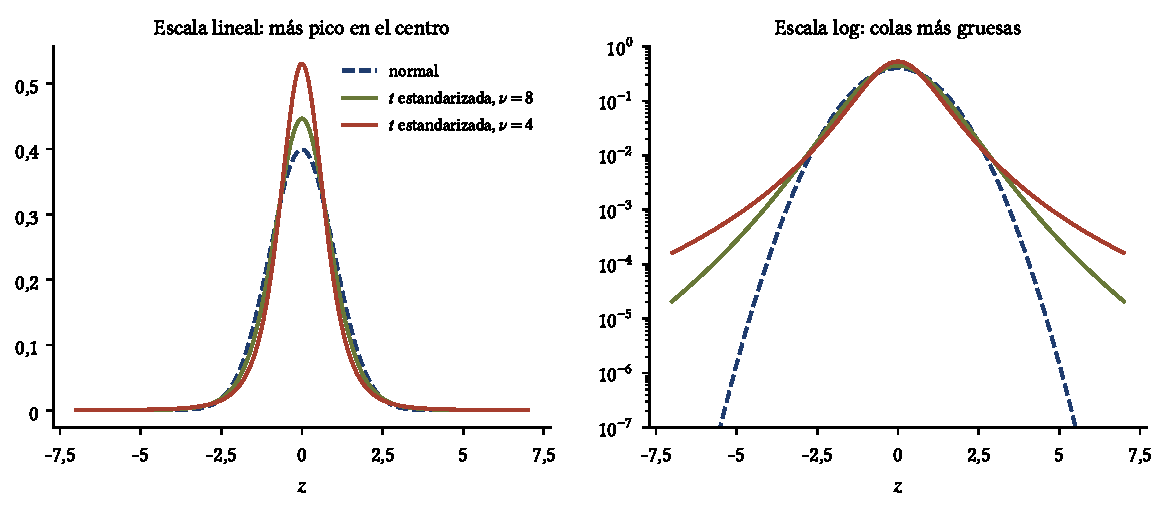
\includegraphics[width=\linewidth]{graficos/cap08_fig_t_student.pdf}
\caption{Densidad de la $t$ de Student estandarizada (varianza 1) con $\nu=4$ y $\nu=8$ frente a la normal
estándar, en escala lineal (izquierda) y logarítmica (derecha).}
\label{fig:tstudentstd}
\end{figure}

\subsection{Cuasi máxima verosimilitud y errores estándar robustos}

¿Qué pasa si se maximiza la verosimilitud normal pero $z_t$ no es normal? Bollerslev y Wooldridge (1992)
mostraron que, si las ecuaciones de la media y la varianza están bien especificadas, el estimador sigue siendo
consistente y asintóticamente normal: es un estimador de \emph{cuasi máxima verosimilitud} (QMLE). Lo que
cambia es su varianza, que toma la forma de ``sándwich'':
\begin{align*}
  \widehat{\Var}(\hat\theta) &= \hat H^{-1}\hat S\,\hat H^{-1},\\
  \hat H &= -\sum_{t=1}^{T}\frac{\partial^2\ell_t(\hat\theta)}{\partial\theta\,\partial\theta'},\\
  \hat S &= \sum_{t=1}^{T}\frac{\partial\ell_t(\hat\theta)}{\partial\theta}\,
            \frac{\partial\ell_t(\hat\theta)}{\partial\theta'} .
\end{align*}
Si el modelo está bien especificado, la igualdad de la información asegura $H=S$ en el límite, y el sándwich
se reduce a $\hat H^{-1}$, la varianza clásica. Con datos financieros conviene reportar siempre la versión
robusta. Calculamos las derivadas numéricamente, con diferencias centrales.

% ---------------------------------------------------------------------
\section{Pruebas de efectos ARCH}
% ---------------------------------------------------------------------

Por la Proposición~\ref{prop:arch1}(iii), bajo un ARCH($q$) los cuadrados $\varepsilon_t^2$ siguen un AR($q$).
Engle (1982) propuso estimar por MCO
\[
  \hat\varepsilon_t^2=a_0+a_1\hat\varepsilon_{t-1}^2+\dots+a_q\hat\varepsilon_{t-q}^2+u_t
\]
y contrastar $H_0:a_1=\dots=a_q=0$ (no hay efectos ARCH) con el estadístico de multiplicadores de Lagrange
\[
  LM=(T-q)\,R^2\ \xrightarrow{d}\ \chi^2_q ,
\]
donde $R^2$ es el de la regresión auxiliar y $T-q$ el número de observaciones que usa. Una alternativa es la
prueba de Ljung-Box aplicada a los cuadrados (McLeod y Li, 1983). Las dos pruebas se aplican también a los
residuos estandarizados $\hat z_t=\hat\varepsilon_t/\hat\sigma_t$ de un modelo estimado: si el modelo capturó la
dinámica de la varianza, $\hat z_t^2$ no debería estar autocorrelacionado.

% ---------------------------------------------------------------------
\section{Evaluación de pronósticos de varianza}
% ---------------------------------------------------------------------

La varianza no se observa, así que los pronósticos $h_t$ se comparan con una aproximación ruidosa, el cuadrado
del rendimiento: $\E_{t-1}[\varepsilon_t^2]=\sigma_t^2$, pero $\varepsilon_t^2=\sigma_t^2z_t^2$ varía mucho
alrededor de $\sigma_t^2$. Patton (2011) muestra que solo algunas funciones de pérdida ordenan bien los
pronósticos con una aproximación ruidosa; dos de ellas son el error cuadrático medio (ECM) y la pérdida QLIKE:
\begin{align*}
  L^{\text{ECM}}(\varepsilon_t^2,h_t)   &= (\varepsilon_t^2-h_t)^2,\\
  L^{\text{QLIKE}}(\varepsilon_t^2,h_t) &= \ln h_t+\frac{\varepsilon_t^2}{h_t}.
\end{align*}

\begin{proposicion}[QLIKE premia el pronóstico correcto]\label{prop:qlike}
Para un pronóstico $h>0$ fijo en $t-1$, $\E_{t-1}\bigl[L^{\text{QLIKE}}(\varepsilon_t^2,h)\bigr]$ se minimiza en
$h=\sigma_t^2$.
\end{proposicion}

\begin{proof}
Como $h$ es conocido en $t-1$:
\begin{align*}
  g(h) &= \E_{t-1}\Bigl[\ln h+\frac{\varepsilon_t^2}{h}\Bigr]\\
       &= \ln h+\frac{\sigma_t^2}{h}.
\end{align*}
Derivamos e igualamos a cero:
\begin{align*}
  g'(h) &= \frac1h-\frac{\sigma_t^2}{h^2}=0,\\
  h     &= \sigma_t^2 .
\end{align*}
Es un mínimo porque la segunda derivada en ese punto es positiva:
\begin{align*}
  g''(h) &= -\frac1{h^2}+\frac{2\sigma_t^2}{h^3},\\
  g''(\sigma_t^2) &= -\frac1{\sigma_t^4}+\frac{2}{\sigma_t^4}\\
                  &= \frac1{\sigma_t^4}>0 . && \qedhere
\end{align*}
\end{proof}

El ECM penaliza los errores en términos absolutos, de modo que unos pocos días de turbulencia dominan el
promedio; QLIKE penaliza los errores relativos y es más estable. Además se usa la \emph{regresión de
Mincer-Zarnowitz}, $\varepsilon_t^2=a+b\,h_t+u_t$: un pronóstico insesgado tiene $a=0$ y $b=1$. Su $R^2$ es
siempre bajo porque $z_t^2$ es muy ruidoso, aunque el pronóstico sea perfecto (Andersen y Bollerslev, 1998).
Para comparar dos modelos se aplica la prueba de Diebold-Mariano del Capítulo~\ref{cap:arma} a la diferencia de
pérdidas.

% ---------------------------------------------------------------------
\section{Ejercicios resueltos}
% ---------------------------------------------------------------------

\begin{ejresuelto}{¿Hay efectos ARCH en el Brent y en el S\&P 500?}\label{ej:archlm}
\enunciado Para los rendimientos diarios del Brent (1987--2026) y mensuales del S\&P 500 (1871--2026), calcule
las primeras autocorrelaciones de $r_t$ y de $r_t^2$ (usando desviaciones respecto de la media), la prueba de
Ljung-Box con 10 rezagos para ambos y la prueba LM de Engle con 5 rezagos.

\solucion
\paso{Paso 1. Autocorrelaciones.} En el Brent, las autocorrelaciones de $r_t$ están entre $-0{,}026$ y
$0{,}015$, mientras que la de $r_t^2$ en el rezago 1 es $0{,}334$ y las siguientes, entre $0{,}053$ y $0{,}075$,
son todas mayores que la banda $\pm0{,}021$. En el S\&P 500 mensual, $r_t^2$ tiene autocorrelaciones de
$0{,}129$, $0{,}155$, $0{,}086$, $0{,}279$ y $0{,}049$ (banda $\pm0{,}045$).

\paso{Paso 2. Pruebas.}
\begin{center}\small
\begin{tabular}{@{}lrrrr@{}}
\toprule
Serie & $Q(10)$ de $r_t$ & $Q(10)$ de $r_t^2$ & $R^2$ auxiliar & LM(5) \\
\midrule
Brent diario      & 25,74 & 1\,718,56 & 0,1199 & 1\,092,93 \\
S\&P 500 mensual  & 168,92 & 450,24 & 0,1002 & 186,61 \\
\bottomrule
\end{tabular}
\end{center}
Para el Brent, el estadístico LM es
\begin{align*}
  LM &= (T-q)\,R^2\\
     &= (9\,121-5)\times0{,}1199\\
     &= 9\,116\times0{,}1199\\
     &\approx 1\,093,
\end{align*}
frente a un valor crítico $\chi^2_5$ al 5\,\% de $11{,}07$. El valor $p$ es del orden de $10^{-234}$.

\paso{Paso 3. Interpretación.} Las dos series rechazan con enorme holgura la ausencia de efectos ARCH. El
$Q(10)$ de $r_t$ del Brent ($p=0{,}004$) también rechaza, pero eso es un espejismo: la prueba clásica supone
homocedasticidad, y la versión robusta del Ejercicio~\ref{ej:acfrob} dio $Q^*(10)=4{,}67$ ($p=0{,}91$). En el
S\&P 500 mensual, la autocorrelación de $0{,}274$ en $r_t$ es el efecto de Working: los precios de la base de
Shiller son promedios mensuales (Capítulo~\ref{cap:arma}).

\codigoweb{cap08_ej01}
\salidaR{cap08_ej01_R.txt}
\lectura{cap08_ej01}

\RvsPy La prueba LM se programa como una regresión auxiliar en los dos lenguajes; Python la comprueba con
\texttt{het\_arch} de \texttt{statsmodels}, que coincide. En R, \texttt{Box.test} devuelve un valor $p$ de cero
cuando es menor que la precisión de la máquina; por eso lo calculamos con \texttt{pchisq(..., lower.tail =
FALSE)}, que trabaja con la cola superior y no pierde precisión.

\begin{figure}[ht]
\centering
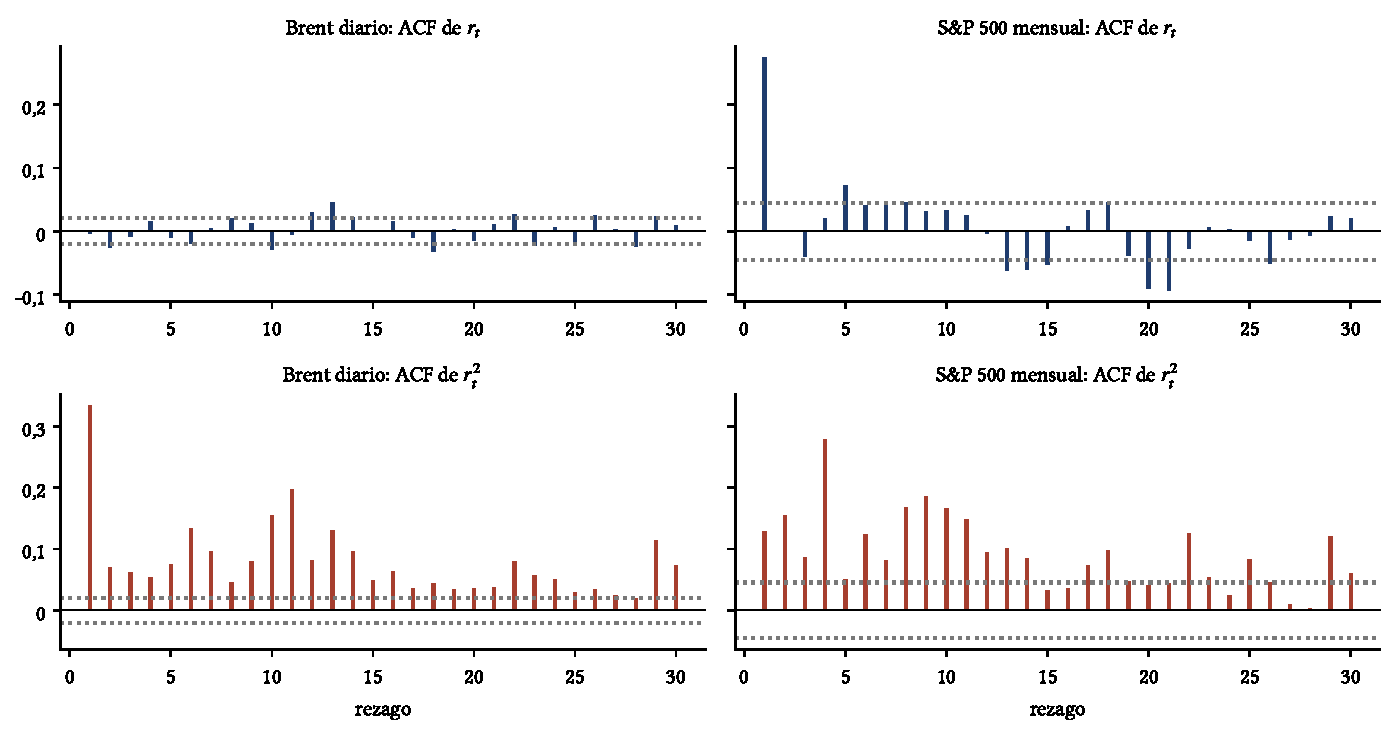
\includegraphics[width=\linewidth]{graficos/cap08_ej01_acf.pdf}
\caption{ACF de los rendimientos (arriba) y de sus cuadrados (abajo) para el Brent diario y el S\&P 500 mensual,
con la banda $\pm1{,}96/\sqrt T$. Los rendimientos del Brent casi no tienen autocorrelación; sus cuadrados sí,
y de forma persistente.}
\label{fig:archacf}
\end{figure}

\begin{conclusion}
Los dos mercados, a frecuencias muy distintas, muestran el patrón que motiva este capítulo: rendimientos casi
impredecibles en nivel y fuertemente predecibles en magnitud.
\end{conclusion}
\end{ejresuelto}

\begin{ejresuelto}{GARCH(1,1) para el Brent, programado a mano}\label{ej:garchn}
\enunciado Estime por máxima verosimilitud un GARCH(1,1) con media constante e innovaciones normales para los
rendimientos diarios del Brent en porcentaje. Programe la verosimilitud y calcule los errores estándar clásicos
(hessiana) y robustos (sándwich). Calcule la persistencia, la vida media, la varianza incondicional implícita y
la condición de cuarto momento. Compare con \texttt{arch}.

\solucion
\paso{Paso 1. Estimación.} El máximo de la log-verosimilitud es $\hat\ell=-20\,074{,}21$, con
\begin{center}\small
\begin{tabular}{@{}lrrrrr@{}}
\toprule
 & Coeficiente & ee hessiana & $t$ & ee robusto & $t$ robusto \\
\midrule
$\mu$      & 0,0346 & 0,0195 & 1,77 & 0,0202 & 1,72 \\
$\omega$   & 0,0517 & 0,0085 & 6,05 & 0,0128 & 4,04 \\
$\alpha$   & 0,0902 & 0,0055 & 16,48 & 0,0094 & 9,64 \\
$\beta$    & 0,9074 & 0,0053 & 172,29 & 0,0087 & 104,79 \\
\bottomrule
\end{tabular}
\end{center}
Los errores robustos son entre 1,5 y 1,7 veces los clásicos en $\omega$, $\alpha$ y $\beta$: las innovaciones no
son normales (lo confirmará el Ejercicio~\ref{ej:garcht}), y la varianza clásica subestima la incertidumbre.

\paso{Paso 2. Persistencia y vida media.}
\begin{align*}
  \hat\phi &= \hat\alpha+\hat\beta\\
           &= 0{,}0902+0{,}9074\\
           &= 0{,}99766,\\[4pt]
  h_{1/2}  &= \frac{\ln0{,}5}{\ln0{,}99766}\\
           &= \frac{-0{,}6931}{-0{,}00234}\\
           &\approx 296 \text{ días}.
\end{align*}
Un choque de volatilidad tarda más de un año bursátil en reducirse a la mitad.

\paso{Paso 3. Varianza incondicional.}
\begin{align*}
  \hat{\bar\sigma}^2 &= \frac{\hat\omega}{1-\hat\alpha-\hat\beta}\\
                     &= \frac{0{,}0517}{0{,}00234}\\
                     &= 22{,}11,
\end{align*}
es decir, una volatilidad anual de $\sqrt{252\times22{,}11}=74{,}6$\,\%, muy por encima de la varianza muestral
($7{,}31$; volatilidad anual de 42,9\,\%). La discrepancia es una advertencia: cuando $\alpha+\beta$ está tan
cerca de uno, $\bar\sigma^2$ es el cociente de dos números pequeños y se estima con muy poca precisión; además,
el modelo atribuye a la varianza de largo plazo los episodios extremos de 2020 y de 2026.

\paso{Paso 4. Cuarto momento.}
\begin{align*}
  (\hat\alpha+\hat\beta)^2+2\hat\alpha^2 &= 0{,}99766^2+2(0{,}0902)^2\\
                                         &= 0{,}99533+0{,}01628\\
                                         &= 1{,}0116>1 .
\end{align*}
El modelo estimado implica curtosis infinita: es el punto rojo de la Figura~\ref{fig:region}.

\paso{Paso 5. La trayectoria de la volatilidad.} Omitiendo el primer año, que depende del valor inicial, la
volatilidad anualizada $\sqrt{252\,\hat\sigma_t^2}$ va de un mínimo de 14,8\,\% (5 de junio de 2014) a un máximo
de 395\,\% (23 de abril de 2020). Dos días antes, en pleno colapso de la demanda por la pandemia, el Brent
había pasado de 17,36 a 9,12 dólares en una sola sesión, un rendimiento logarítmico de $-64$\,\%, y al día
siguiente subió a 13,77 (Figura~\ref{fig:garchvol}).

\codigoweb{cap08_ej02}
\salidaR{cap08_ej02_R.txt}
\lectura{cap08_ej02}

\RvsPy Las dos implementaciones recorren la misma recursión con un bucle explícito y usan el mismo valor
inicial que \texttt{arch}, por lo que los tres resultados coinciden en todas las cifras mostradas. Los
optimizadores sí difieren: en R usamos \texttt{nlminb}, que llegó al mismo máximo que \texttt{arch} con más
precisión que \texttt{optim(method = "L-BFGS-B")}; en Python, \texttt{minimize} de \texttt{scipy} con
\texttt{L-BFGS-B}. Con ambos conviene fijar tolerancias estrictas, porque la verosimilitud es muy plana en la
dirección de $\omega/(1-\alpha-\beta)$. La hessiana y los scores se calculan con las mismas diferencias
centrales en los dos lenguajes.

\begin{figure}[ht]
\centering
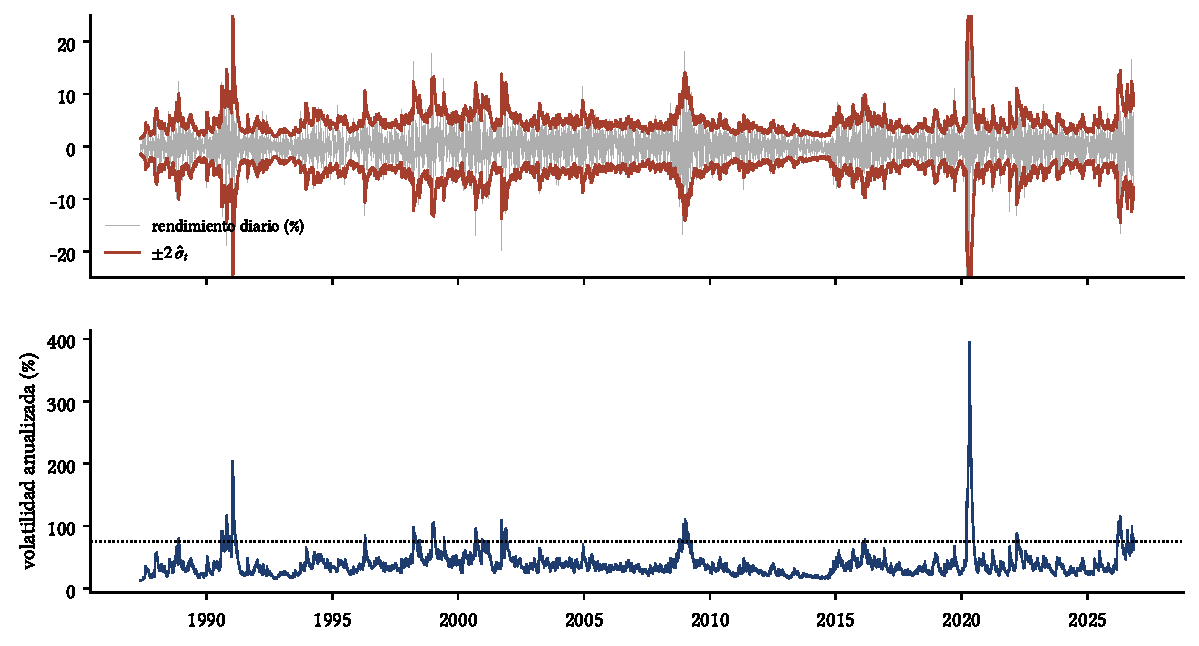
\includegraphics[width=\linewidth]{graficos/cap08_ej02_volatilidad.pdf}
\caption{Arriba: rendimientos diarios del Brent con las bandas $\pm2\hat\sigma_t$ del GARCH(1,1) (eje recortado a
$\pm25$\,\%). Abajo: volatilidad anualizada estimada; la línea punteada es la implícita en $\hat{\bar\sigma}^2$.}
\label{fig:garchvol}
\end{figure}

\begin{conclusion}
El GARCH(1,1) reproduce el agrupamiento de volatilidad del Brent con tres parámetros. La volatilidad es muy
persistente ($\alpha+\beta=0{,}998$) y varía enormemente en el tiempo: decir que ``la volatilidad del petróleo
es de 43\,\% anual'' oculta que ha oscilado entre 15\,\% y casi 400\,\%.
\end{conclusion}
\end{ejresuelto}

\begin{ejresuelto}{Innovaciones $t$ de Student y diagnóstico}\label{ej:garcht}
\enunciado Reestime el modelo con innovaciones $t$ de Student estandarizadas. Compare con el modelo normal
mediante AIC y BIC. Calcule los residuos estandarizados $\hat z_t=(r_t-\hat\mu)/\hat\sigma_t$ y compare su
asimetría, curtosis, prueba de Jarque-Bera y pruebas de Ljung-Box con las de los rendimientos originales.

\solucion
\paso{Paso 1. Estimación.} Con errores robustos:
\begin{center}\small
\begin{tabular}{@{}lrrr@{}}
\toprule
 & Coeficiente & ee robusto & $t$ \\
\midrule
$\mu$    & 0,0522 & 0,0184 & 2,83 \\
$\omega$ & 0,0593 & 0,0118 & 5,03 \\
$\alpha$ & 0,0832 & 0,0074 & 11,24 \\
$\beta$  & 0,9123 & 0,0072 & 127,41 \\
$\nu$    & 5,2295 & 0,2784 & 18,78 \\
\bottomrule
\end{tabular}
\end{center}
La persistencia baja a $0{,}99554$ (vida media de 155 días). Con $\hat\nu=5{,}23$, la curtosis de la $t$
estandarizada es
\begin{align*}
  3+\frac{6}{\hat\nu-4} &= 3+\frac{6}{1{,}2295}\\
                        &= 7{,}88 .
\end{align*}

\paso{Paso 2. Comparación.}
\begin{center}\small
\begin{tabular}{@{}lrrr@{}}
\toprule
Modelo & $\hat\ell$ & AIC & BIC \\
\midrule
GARCH normal & $-20\,074{,}21$ & 40\,156,43 & 40\,184,90 \\
GARCH-$t$    & $-19\,752{,}61$ & 39\,515,21 & 39\,550,81 \\
\bottomrule
\end{tabular}
\end{center}
El parámetro adicional aumenta la log-verosimilitud en $321{,}6$ puntos, y los dos criterios prefieren la $t$
por más de 600 puntos. (Una prueba de razón de verosimilitudes no es estándar aquí, porque la normal
corresponde a $\nu=\infty$, en la frontera del espacio de parámetros; pero con una diferencia de esta
magnitud no hace falta.)

\paso{Paso 3. Diagnóstico.}
\begin{center}\small
\begin{tabular}{@{}lrrrrr@{}}
\toprule
Serie & Asimetría & Curtosis & Jarque-Bera & $Q(10)$ nivel & $Q(10)$ cuadrados \\
\midrule
$r_t$        & $-1{,}49$ & 55,97 & 1\,069\,541 & 25,74 & 1\,718,56 \\
$\hat z_t$   & $-0{,}20$ & 5,48 & 2\,388 & 22,64 & 14,93 \\
\bottomrule
\end{tabular}
\end{center}
El modelo absorbe casi toda la dependencia de los cuadrados: $Q(10)$ baja de $1\,718{,}56$ a $14{,}93$
($p=0{,}135$). La curtosis cae de 56 a 5,5: la mayor parte de las colas gruesas de los rendimientos se explica
por la volatilidad cambiante. Lo que queda (una curtosis de 5,5, aún mayor que 3) es lo que la $t$ de Student
modela. Persiste una autocorrelación débil en el nivel ($p=0{,}012$), que se concentra en el rezago 2 y
podría modelarse con un término AR en la media, aunque su tamaño ($-0{,}026$) es económicamente irrelevante.

\paso{Paso 4. Las colas.} Hay $0{,}00362\times9\,121=33$ días con $|\hat z_t|>4$. La normal predice
$6{,}33\times10^{-5}\times9\,121=0{,}58$ días; la $t$ con $\nu=5{,}23$, $0{,}00335\times9\,121=31$ días. El
gráfico cuantil-cuantil de la Figura~\ref{fig:garchqq} lo muestra: frente a la normal los puntos se curvan en
los extremos; frente a la $t$ siguen la diagonal.

\codigoweb{cap08_ej03}
\salidaR{cap08_ej03_R.txt}
\lectura{cap08_ej03}

\RvsPy La función \texttt{lgamma} de R equivale a \texttt{gammaln} de \texttt{scipy.special}; se usan los
logaritmos de la función gamma para evitar desbordamientos. En Python, \texttt{stats.t.ppf(u, nu)} da los
cuantiles de la $t$ sin estandarizar, que multiplicamos por $\sqrt{(\nu-2)/\nu}$ para el gráfico.

\begin{figure}[ht]
\centering
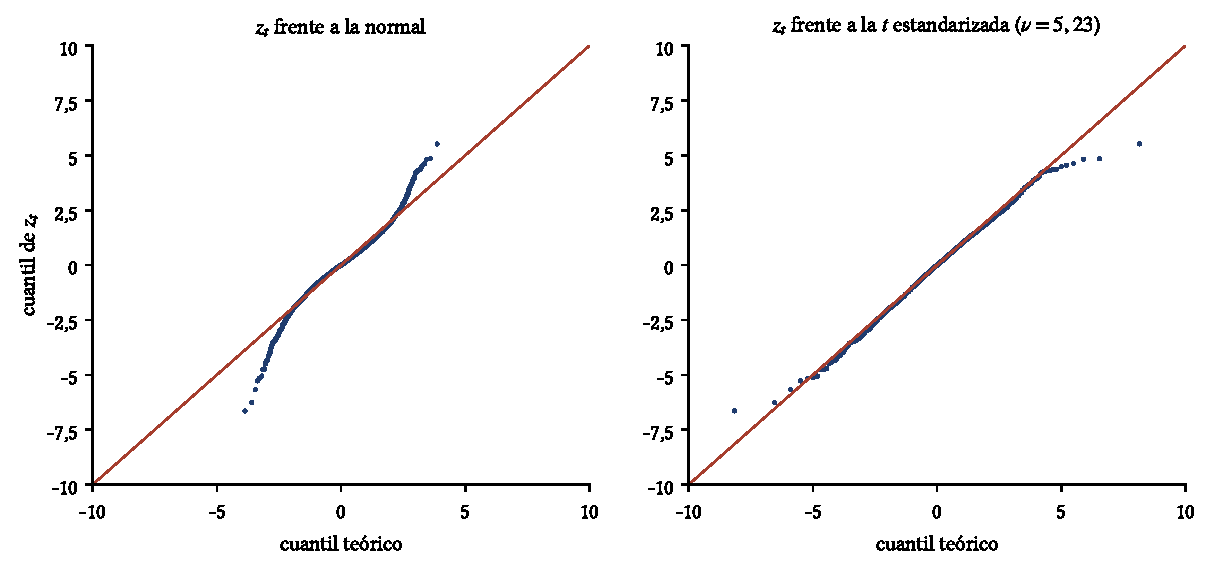
\includegraphics[width=\linewidth]{graficos/cap08_ej03_qq.pdf}
\caption{Gráficos cuantil-cuantil de los residuos estandarizados del GARCH-$t$ frente a la normal (izquierda) y
frente a la $t$ estandarizada con $\hat\nu=5{,}23$ (derecha).}
\label{fig:garchqq}
\end{figure}

\begin{conclusion}
Las innovaciones normales no bastan para el Brent: aun condicionando en la volatilidad, los choques extremos son
más frecuentes de lo que permite la normal. La $t$ de Student, con un solo parámetro adicional, reproduce bien
las colas y mejora drásticamente la verosimilitud.
\end{conclusion}
\end{ejresuelto}

\begin{ejresuelto}{Pronóstico de la volatilidad del Brent}\label{ej:garchpron}
\enunciado Con el GARCH-$t$ estimado con toda la muestra, pronostique la varianza del Brent para los próximos
252 días hábiles a partir del 3 de noviembre de 2026. Calcule la volatilidad de un mes (21 días) y de un año
(252 días), y compárelas con la regla de la raíz del tiempo.

\solucion
\paso{Paso 1. La varianza de mañana.} El último rendimiento es $r_T=-0{,}336$\,\%, de modo que
$\hat\varepsilon_T^2=(r_T-\hat\mu)^2=0{,}1505$, y la varianza estimada para ese día es $\hat\sigma_T^2=24{,}7793$.
Entonces
\begin{align*}
  \hat\sigma_{T+1}^2 &= \hat\omega+\hat\alpha\,\hat\varepsilon_T^2+\hat\beta\,\hat\sigma_T^2\\
                     &= 0{,}0593+0{,}0832\times0{,}1505+0{,}9123\times24{,}7793\\
                     &= 22{,}678,
\end{align*}
una volatilidad diaria de $4{,}76$\,\% y anualizada de $\sqrt{252\times22{,}678}=75{,}6$\,\%. El año 2026 ha
sido excepcional en los datos: el Brent empezó el año en 62 dólares, llegó a 138 en abril y ha tenido
movimientos diarios de más de 10\,\% en ambas direcciones.

\paso{Paso 2. Nivel de largo plazo.}
\begin{align*}
  \hat{\bar\sigma}^2 &= \frac{0{,}0593}{1-0{,}99554}\\
                     &= 13{,}286,
\end{align*}
es decir, 57,9\,\% anual.

\paso{Paso 3. Pronóstico a 21 días.} Por la Proposición~\ref{prop:garchpron}, con $\hat\phi^{20}=0{,}9145$:
\begin{align*}
  \E_T[\sigma_{T+21}^2] &= 13{,}286+0{,}9145\times(22{,}678-13{,}286)\\
                        &= 13{,}286+0{,}9145\times9{,}392\\
                        &= 13{,}286+8{,}589\\
                        &= 21{,}874 .
\end{align*}
La siguiente tabla resume la trayectoria:
\begin{center}\small
\begin{tabular}{@{}rrr@{}}
\toprule
$h$ (días) & $\E_T[\sigma^2_{T+h}]$ & Volatilidad anualizada \\
\midrule
1   & 22,678 & 75,6\,\% \\
21  & 21,874 & 74,2\,\% \\
63  & 20,404 & 71,7\,\% \\
126 & 18,657 & 68,6\,\% \\
252 & 16,344 & 64,2\,\% \\
\bottomrule
\end{tabular}
\end{center}

\paso{Paso 4. Volatilidad acumulada.} Por el Corolario~\ref{cor:varH}, con $(1-\hat\phi^{21})/(1-\hat\phi)=20{,}089$:
\begin{align*}
  \sum_{h=1}^{21}\E_T[\sigma_{T+h}^2] &= 21\times13{,}286+9{,}392\times20{,}089\\
                                      &= 279{,}01+188{,}67\\
                                      &= 467{,}68,\\[4pt]
  \sqrt{467{,}68} &= 21{,}63 .
\end{align*}
La volatilidad del mes es, por tanto, de 21,63\,\%. La regla de la raíz daría $\sqrt{21\times22{,}678}=21{,}82$\,\%, casi lo mismo. A un año, en cambio, el GARCH da
una volatilidad de $\sqrt{4\,771}=69{,}07$\,\% frente a $75{,}60$\,\% de la regla: como la volatilidad actual está
por encima de su nivel normal, la regla de la raíz sobreestima el riesgo de largo plazo.

\codigoweb{cap08_ej04}
\salidaR{cap08_ej04_R.txt}
\lectura{cap08_ej04}

\RvsPy El método \texttt{forecast} de \texttt{arch} implementa la misma fórmula y coincide con nuestro cálculo
(las diferencias en la tercera decimal a 252 días vienen de diferencias mínimas en los parámetros que
encuentran los optimizadores, que la potencia $\hat\phi^{\,h}$ amplifica). En Python, la figura sitúa los
pronósticos en días hábiles futuros con \texttt{pd.bdate\_range}.

\begin{figure}[ht]
\centering
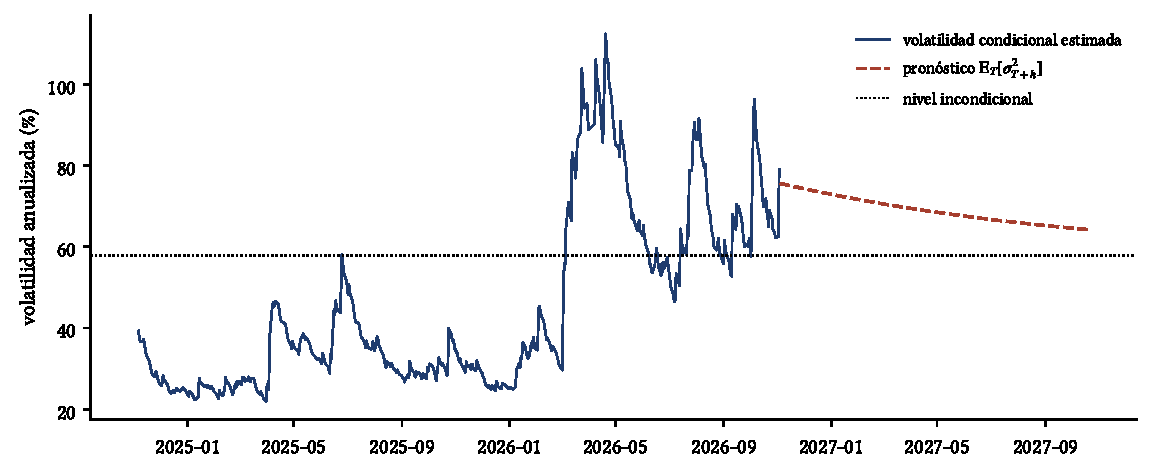
\includegraphics[width=0.92\linewidth]{graficos/cap08_ej04_pronostico.pdf}
\caption{Volatilidad condicional anualizada del Brent en los dos últimos años de la muestra y su pronóstico a
252 días hábiles. El pronóstico desciende lentamente hacia el nivel incondicional (línea punteada).}
\label{fig:garchpron}
\end{figure}

\begin{conclusion}
Con una persistencia de $0{,}9955$, el pronóstico de volatilidad del Brent desciende despacio: un año después
todavía está por encima de su nivel de largo plazo. Para horizontes de días, la regla de la raíz es una buena
aproximación; para horizontes de meses, conviene usar el pronóstico del modelo.
\end{conclusion}
\end{ejresuelto}

\begin{ejresuelto}{¿Pronostica mejor el GARCH? Evaluación fuera de muestra}\label{ej:garchfuera}
\enunciado Estime un GARCH(1,1) normal con los datos del Brent hasta el 31 de diciembre de 2015 y, con esos
parámetros fijos, genere pronósticos a un día para 2016--2026. Compárelos con la EWMA de RiskMetrics
($\lambda=0{,}94$) y con la varianza histórica de los 250 días previos, usando ECM, QLIKE, la regresión de
Mincer-Zarnowitz y la prueba de Diebold-Mariano sobre QLIKE.

\solucion
\paso{Paso 1. Estimación.} Con 6\,370 días, $\hat\omega=0{,}0265$, $\hat\alpha=0{,}0697$ y $\hat\beta=0{,}9300$:
la persistencia dentro de la muestra es $0{,}9997$, casi un IGARCH. La muestra de evaluación tiene 2\,751 días
(4 de enero de 2016 a 3 de noviembre de 2026).

\paso{Paso 2. Pérdidas.}
\begin{center}\small
\begin{tabular}{@{}lrrrrr@{}}
\toprule
Modelo & ECM & QLIKE & $a$ (MZ) & $b$ (MZ) & $R^2$ (MZ) \\
\midrule
GARCH(1,1)          & 7\,947,35 & 2,7237 & 2,530 & 0,736 & 0,0664 \\
EWMA                & 7\,967,32 & 2,7454 & 2,673 & 0,747 & 0,0626 \\
Ventana de 250 días & 8\,476,37 & 3,0766 & 6,552 & 0,386 & 0,0032 \\
\bottomrule
\end{tabular}
\end{center}
El GARCH tiene la menor pérdida con los dos criterios; la EWMA queda muy cerca y la ventana móvil, lejos.

\paso{Paso 3. Diebold-Mariano.} Con $d_t=L_t^{\text{rival}}-L_t^{\text{GARCH}}$ en QLIKE y errores de
Newey-West:
\begin{center}\small
\begin{tabular}{@{}lrr@{}}
\toprule
Comparación & $\bar d$ & $t$ \\
\midrule
GARCH frente a EWMA        & 0,0217 & 3,70 \\
GARCH frente a ventana 250 & 0,3529 & 3,73 \\
\bottomrule
\end{tabular}
\end{center}
Las dos diferencias son significativas: el GARCH pronostica mejor. La ventaja sobre la EWMA es pequeña en nivel
(menos del 1\,\% de la pérdida media), pero sistemática.

\paso{Paso 4. Mincer-Zarnowitz.} Ningún modelo es insesgado: $\hat b<1$ indica que, cuando pronostican varianzas
altas, la realizada promedio es menor (sobrerreaccionan a los choques). La ventana móvil es la peor: su
$\hat b=0{,}386$ y su $R^2$ de $0{,}003$ revelan que apenas sigue a la volatilidad. Los $R^2$ bajos de todos los
modelos son los esperables con un aproximante tan ruidoso como $\varepsilon_t^2$.

\codigoweb{cap08_ej05}
\salidaR{cap08_ej05_R.txt}
\lectura{cap08_ej05}

\RvsPy Los pronósticos fuera de muestra se obtienen haciendo correr la recursión del GARCH sobre toda la
serie con los parámetros fijos: $\hat\sigma_t^2$ solo usa datos hasta $t-1$, así que no hay mirada al futuro. Lo
mismo vale para la EWMA y para la ventana móvil, que en R y en Python se calculan con bucles idénticos.

\begin{figure}[ht]
\centering
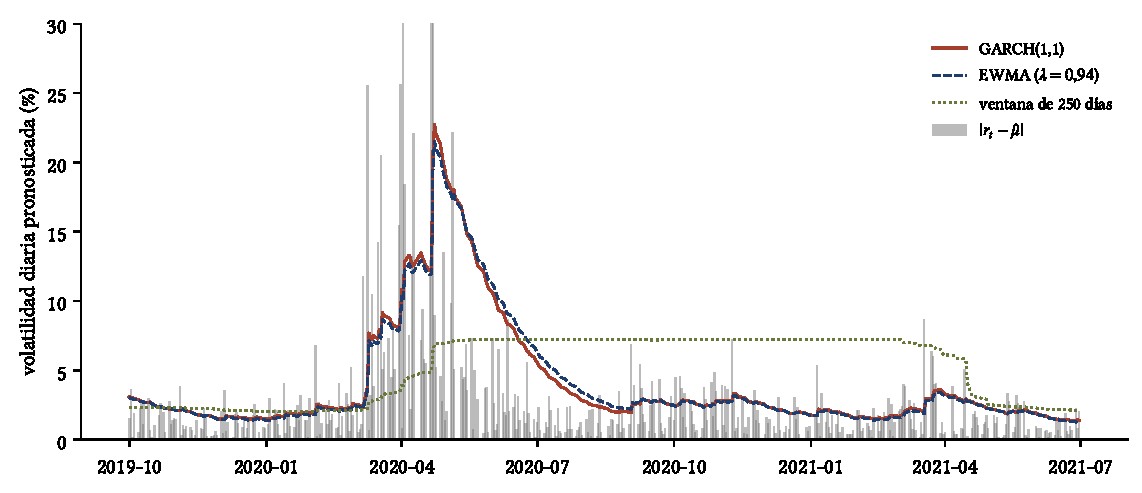
\includegraphics[width=0.92\linewidth]{graficos/cap08_ej05_fuera_muestra.pdf}
\caption{Pronósticos de volatilidad diaria del Brent entre octubre de 2019 y junio de 2021, frente al valor
absoluto del rendimiento (barras). El GARCH y la EWMA reaccionan en pocos días al choque de 2020; la ventana de
250 días reacciona tarde y se mantiene alta durante un año, hasta que el choque sale de la ventana.}
\label{fig:garchfuera}
\end{figure}

\begin{conclusion}
Fuera de muestra, el GARCH(1,1) supera con significancia a la EWMA y a la varianza histórica. La ventana móvil
es la peor por construcción: pondera igual un dato de hace once meses que uno de ayer, y deja de recordar un
choque de golpe. La EWMA, que no requiere estimación, es una alternativa casi tan buena como el GARCH.
\end{conclusion}
\end{ejresuelto}

% ---------------------------------------------------------------------
\section{Ejercicios propuestos}
% ---------------------------------------------------------------------

\begin{enumerate}[label=\textbf{\thechapter.\arabic*},leftmargin=*,itemsep=6pt]
  \item Para un ARCH(1) normal con $\omega=0{,}2$ y $\alpha=0{,}3$, calcule la varianza incondicional y la
  curtosis. \textit{Respuesta: $0{,}2857$ y $3{,}740$.}

  \item Para un GARCH(1,1) normal con $\omega=0{,}02$, $\alpha=0{,}05$ y $\beta=0{,}93$, calcule la varianza
  incondicional, la vida media y la curtosis. \textit{Respuesta: $1$; $34{,}3$ períodos; $3{,}434$.}

  \item Bollerslev (1988) muestra que, en un GARCH(1,1), la primera autocorrelación de $\varepsilon_t^2$ es
  $\rho_1=\alpha(1-\alpha\beta-\beta^2)/(1-2\alpha\beta-\beta^2)$. Calcúlela con los parámetros del ejercicio
  anterior y verifíquela simulando dos millones de observaciones. \textit{Respuesta: $0{,}105$.}

  \item Demuestre que en la EWMA el pronóstico de la varianza es plano:
  $\E_T[\sigma_{T+h}^2]=\sigma_{T+1}^2$ para todo $h\ge1$. ¿Qué implica para la regla de la raíz del tiempo?

  \item Demuestre que la pérdida ECM también se minimiza en $h=\sigma_t^2$. ¿Por qué entonces se prefiere QLIKE
  cuando hay días de turbulencia extrema?

  \item Demuestre que la varianza de un ARCH(2) es $\omega/(1-\alpha_1-\alpha_2)$ y escriba $\varepsilon_t^2$
  como un AR(2).

  \item \emph{(Con datos del BCRP.)} Estime un GARCH(1,1)-$t$ para los rendimientos diarios del tipo de cambio
  interbancario sol/dólar. Compare la persistencia y los grados de libertad con los del Brent. ¿Cómo se refleja
  la intervención cambiaria del BCRP en la volatilidad estimada?

  \item \emph{(Simulación.)} Simule 500 muestras de $T=2\,000$ observaciones de un GARCH(1,1)-$t$ con los
  parámetros del Ejercicio~\ref{ej:garcht} y reestime el modelo en cada una con su función propia. Dibuje la
  distribución de $\hat\alpha+\hat\beta$ y de $\hat\nu$. ¿Están sesgadas?

  \item \emph{(Con datos.)} Repita el Ejercicio~\ref{ej:garchfuera} con el GARCH-$t$ y reestimando los
  parámetros cada año con una ventana creciente. ¿Cambia la clasificación de los modelos?
\end{enumerate}

% ---------------------------------------------------------------------
\section{Resumen de fórmulas}
% ---------------------------------------------------------------------

\begin{table}[H]
\centering\small
\begin{tabular}{@{}ll@{}}
\toprule
Concepto & Fórmula \\
\midrule
ARCH(1) & $\sigma^2=\omega/(1-\alpha)$;\quad $\kappa=3(1-\alpha^2)/(1-3\alpha^2)$ \\
GARCH(1,1) & $\sigma_t^2=\omega+\alpha\varepsilon_{t-1}^2+\beta\sigma_{t-1}^2$;\quad $\bar\sigma^2=\omega/(1-\alpha-\beta)$ \\
Curtosis GARCH(1,1) & $\kappa=3[1-(\alpha+\beta)^2]/[1-(\alpha+\beta)^2-2\alpha^2]$ \\
EWMA & $\sigma_t^2=\lambda\sigma_{t-1}^2+(1-\lambda)\varepsilon_{t-1}^2$,\quad $\lambda=0{,}94$ \\
Pronóstico & $\E_T[\sigma_{T+h}^2]=\bar\sigma^2+(\alpha+\beta)^{h-1}(\sigma_{T+1}^2-\bar\sigma^2)$ \\
Vida media & $h_{1/2}=\ln0{,}5/\ln(\alpha+\beta)$ \\
Log-verosimilitud normal & $\ell_t=-\frac12[\ln2\pi+\ln\sigma_t^2+\varepsilon_t^2/\sigma_t^2]$ \\
Varianza QMLE & $\hat H^{-1}\hat S\hat H^{-1}$ \\
Prueba LM de Engle & $(T-q)R^2\sim\chi^2_q$ \\
Pérdida QLIKE & $\ln h_t+\varepsilon_t^2/h_t$ \\
\bottomrule
\end{tabular}
\caption{Fórmulas principales del Capítulo 8.}
\end{table}

\section*{Referencias}
\begin{itemize}[leftmargin=*]
  \item Andersen, T. G. y Bollerslev, T. (1998). Answering the skeptics: Yes, standard volatility models do
        provide accurate forecasts. \emph{International Economic Review}, 39(4), 885--905.
  \item Bollerslev, T. (1986). Generalized autoregressive conditional heteroskedasticity. \emph{Journal of
        Econometrics}, 31(3), 307--327.
  \item Bollerslev, T. (1988). On the correlation structure for the generalized autoregressive conditional
        heteroskedastic process. \emph{Journal of Time Series Analysis}, 9(2), 121--131.
  \item Bollerslev, T. y Wooldridge, J. M. (1992). Quasi-maximum likelihood estimation and inference in dynamic
        models with time-varying covariances. \emph{Econometric Reviews}, 11(2), 143--172.
  \item Engle, R. F. (1982). Autoregressive conditional heteroscedasticity with estimates of the variance of
        United Kingdom inflation. \emph{Econometrica}, 50(4), 987--1007.
  \item J.\,P.~Morgan/Reuters (1996). \emph{RiskMetrics: Technical Document}, 4.ª ed. Nueva York.
  \item McLeod, A. I. y Li, W. K. (1983). Diagnostic checking ARMA time series models using squared-residual
        autocorrelations. \emph{Journal of Time Series Analysis}, 4(4), 269--273.
  \item Patton, A. J. (2011). Volatility forecast comparison using imperfect volatility proxies.
        \emph{Journal of Econometrics}, 160(1), 246--256.
\end{itemize}
